\documentclass[11pt,twocolumn,a4paper]{article}
\usepackage[top=2.5cm,bottom=2.5cm,left=2.5cm,right=2.5cm,columnsep=0.6cm]{geometry}
\usepackage[T1]{fontenc}
\usepackage{newtxtext,newtxmath}
\usepackage[scaled=0.85]{beramono}
\usepackage{microtype}
\usepackage{booktabs}
\usepackage{graphicx}
\usepackage{xcolor}
\usepackage{amsmath}
\usepackage{enumitem}
\usepackage[authoryear,round]{natbib}
\usepackage[colorlinks=true,citecolor={blue!70!black},linkcolor={blue!70!black},urlcolor={blue!70!black}]{hyperref}
\usepackage{caption}
\usepackage{float}
\captionsetup{font=small,labelfont=small,skip=4pt}
\setlength{\bibsep}{2pt}
\setlength{\textfloatsep}{10pt}
\newcommand{\open}[1]{\textcolor{red}{[OPEN: #1]}}
\newcommand{\cpl}{\Delta_{\text{pose}}}
\newcommand{\src}[1]{\textsc{#1}}
\newcommand{\ib}{\src{informburo}}
\newcommand{\kh}{\src{khabar}}
\newcommand{\qz}{\src{qazaqstantv}}
\renewcommand{\paragraph}[1]{\par\smallskip\noindent\textbf{#1}\hspace{0.5em}}

\title{\vspace{-1.2cm}\bfseries\Large Rewriting the References Helped Pose-Based Kazakh Sign Language\\ Translation More Than Any Model Change}
\author{\textbf{Adilet Tasbolat}\textsuperscript{1} \quad \textbf{Asan Tasmulaev}\textsuperscript{2} \quad \textbf{Zhoshy Khalelov}\textsuperscript{3} \quad \textbf{Rakhat Meiramov}\textsuperscript{1}\\[2pt]
\textsuperscript{1}ISSAI, Nazarbayev University, Astana, Kazakhstan\\
\textsuperscript{2}Secondary School No.~101, Kazakhstan \quad \textsuperscript{3}West Kazakhstan Oblast, Kazakhstan}
\date{\small\textit{Preprint, work in progress.} October 2026}

\begin{document}
\twocolumn[
\maketitle
\vspace{0.6cm}
]

\begin{center}\textbf{Abstract}\end{center}
\vspace{-0.2cm}
{\small\leftskip=0.6cm\rightskip=0.6cm\noindent
We translate Kazakh Sign Language news interpretation into Kazakh text from pose keypoints alone, with a Uni-Sign pose encoder feeding mT5-base, trained on 59k clips from three broadcasters. Across 42 from-scratch runs in twelve configurations, each with its readings fixed before launch, three findings stand. First, training is bimodal. A run either starts reading its pose input (``takes off'', chrF${\approx}30$) or falls back on the decoder's language prior (chrF${\approx}20$), and which one happens is largely chance. Seven of the 36 runs on the original data took off; seeds of one configuration span 10 chrF; and no change to the encoder objective, learning rates, decoder initialisation, frame rate or preprocessing moved the rate. Second, the same checkpoints that almost never write the right sentence (WER 0.96) pick it out of 200 same-source candidates 81\% of the time on the test set, once the text prior is subtracted with pointwise mutual information. Third, the largest gain came from the data. Used as an auditor, retrieval shows that 13\% of one broadcaster's training references describe a different part of the broadcast, an artefact of fuzzy-matching article text to time segments. Removing them changes nothing. Rewriting the references with an LLM so that they cover exactly what was spoken, in the article's wording, does two things. Without retraining, it raises that broadcaster's retrieval from 0.67 to 0.87, so about two thirds of its apparent deficit was evaluation error. Training from scratch on the rewritten references then raises test chrF from 30.3 to 35.8 ($+5.5$, 95\% CI $[4.9, 6.1]$), with gains in every source. The best model gets the story but almost never the rare words (2.6\% recall), and the signers' hands are 31--51 pixels across.
\par}

\section{Introduction}

Sign language translation (SLT) from video is usually reported as one number on one benchmark \citep{camgoz2018nslt,camgoz2020slt}, and recent gloss-free systems put a pretrained visual or pose encoder in front of a pretrained language model \citep{zhou2023gfslt,wong2024sign2gpt,gong2024signllm,li2025unisign}. That recipe hides a failure the NLP literature has long known under other names. A decoder strong enough to write fluent text can learn to ignore its input \citep{bowman2016generating,voita2021analyzing} and produce hallucinated, prior-driven output \citep{lee2018hallucinations}. With a weak input signal, low-resource data and noisy references, one training run cannot show which of these is happening.

This paper is a record of what did and did not improve a keypoints-only translator for Kazakh Sign Language (KSL) news interpretation, built on Uni-Sign \citep{li2025unisign} and mT5 \citep{xue2021mt5}. We started by asking which input representation works best. Running that comparison changed the question. One configuration's three seeds spanned 19.8--29.8 chrF, wider than any difference between configurations, and the spread came from a single binary event: whether the decoder ever starts to read the encoder. Every intervention we then tried on the model side left that event's rate where it was. The changes that mattered came from treating the model as a measuring instrument for the data rather than the other way round.

\paragraph{Contributions.}
(1) Evidence, over 42 from-scratch runs, that gloss-free pose-to-text training is bimodal and that the outcome of a single run is mostly chance. Five families of model-side intervention leave the takeoff rate unchanged (\S\ref{sec:bimodal}). (2) A pose-shuffle measure of encoder use with per-run confidence intervals. It shows coupling is graded below the takeoff threshold, which a binary rule hides (\S\ref{sec:coupling}). (3) A demonstration that the same checkpoints solve sentence retrieval at 81--86\% top-1 out of 200 while generation stays near WER 0.96, with controls for duration, memorisation and coupling (\S\ref{sec:retrieval}). (4) A retrieval-based corpus audit that finds the misaligned references, and an LLM rewrite of them. The rewrite exposes most of one source's deficit as evaluation error and, used for training, gives the only large gain in the study (\S\ref{sec:refs}). (5) A list of pipeline faults that each would have reversed a conclusion without raising an error (Appendix~\ref{app:faults}).

\section{Related Work}

\paragraph{Gloss-free SLT.}
Early neural SLT used gloss supervision \citep{camgoz2018nslt,camgoz2020slt}, which is costly to annotate and a lossy description of signing \citep{muller2023considerations}. Gloss-free systems instead align visual features with text through contrastive pretraining \citep{zhou2023gfslt} or connect a visual encoder to a frozen or tuned LLM \citep{wong2024sign2gpt,gong2024signllm}. Uni-Sign \citep{li2025unisign} pretrains a pose and RGB encoder on 1{,}985 hours of Chinese news interpretation (CSL-News) and fine-tunes it with mT5 for translation. It is our encoder and our template. Large web corpora such as YouTube-ASL \citep{uthus2023youtubeasl} and BOBSL \citep{albanie2021bobsl}, and benchmarks such as How2Sign \citep{duarte2021how2sign} and CSL-Daily \citep{zhou2021csldaily}, show the same broadcast-interpretation setting and its noise.

\paragraph{Kazakh--Russian Sign Language.}
Prior KRSL work covers isolated-sign and linguistic datasets \citep{imashev2020krsl,mukushev2022krslonline}. To our knowledge there is no published continuous KSL-to-Kazakh translation result to compare against. The three-broadcaster corpus used here was collected and segmented at ISSAI and has not been published separately.

\paragraph{Decoders that ignore the encoder.}
Posterior collapse in VAEs \citep{bowman2016generating}, analyses of source versus target contributions in NMT \citep{voita2021analyzing} and NMT hallucination \citep{lee2018hallucinations} all describe a conditional decoder that relies on its own prefix. We measure the sign-language case directly by permuting encoder outputs. To counter the prior at scoring time we use the mutual-information correction from dialogue \citep{li2016mmi} and zero-shot scoring \citep{holtzman2021surface}.

\paragraph{Noisy and misaligned references.}
Noise in parallel data hurts NMT unevenly depending on its type \citep{khayrallah2018noise}. In sign language corpora built from broadcast subtitles, the subtitles are offset from the signing, and \citet{bull2021aligning} learn to re-align them in time. Our noise is different: the text, not its timing, belongs to another part of the broadcast. Rewriting captions with a language model has improved vision--language training \citep{fan2023laclip}. We apply the same idea to sign language references and measure its effect on both training and evaluation. \citet{duarte2022retrieval} study sign video retrieval from free-form text queries; we use retrieval both as a task and as a data-audit tool.

\paragraph{Seed variance.}
Fine-tuning outcomes can depend on the seed as much as on the method \citep{dodge2020finetuning,bouthillier2021variance}. Our bimodal takeoff is an extreme case, and it forces the design used throughout: several seeds per arm, readings fixed in advance, and continuous measures where the binary outcome lacks power.

\section{Setup}

\subsection{Data}
\label{sec:data}

The corpus holds sign language interpretation insets from three Kazakh news broadcasters, segmented into sentence-level clips with Kazakh transcripts and pre-extracted COCO-WholeBody keypoints \citep{jin2020wholebody} from RTMW \citep{jiang2024rtmw}. It totals about 360 hours. The three sources differ in ways that matter later (Table~\ref{tab:data}). \ib{} and \kh{} carry one caption-style transcript per clip. \qz{} stores two: \texttt{text\_asr}, a Whisper transcription \citep{radford2023whisper} of exactly what the anchor said in the clip's window, and \texttt{text\_human}, sentences of the broadcast's web article fuzzy-matched onto time segments. Training used \texttt{text\_human} where a match existed (89.8\%) and \texttt{text\_asr} otherwise.

We rebuilt the splits because the released versions leaked: an archived \qz{} training split shared 563 videos with the recollected dev split, 64\% of dev clips. Canonical splits are assigned per source video by a salted hash: 59{,}008 train clips (10{,}398 videos), 8{,}411 dev (2{,}575) and 8{,}360 test (2{,}534). All model selection uses a frozen \emph{selection set} of 600 dev clips: 200 per source, one per video, stratified over duration quartiles. Test was opened twice, each time for one checkpoint chosen on dev: once for retrieval (\S\ref{sec:retrieval}) and once for the final model (\S\ref{sec:refs}).

\begin{table}[t]
\centering\small
\setlength{\tabcolsep}{4pt}
\begin{tabular}{lrrrl}
\toprule
Source & fps & \% train & hand px & reference \\
\midrule
\ib & 50 & 9 & 34 & caption \\
\kh & 25 & 36 & 51 & caption \\
\qz & 30 & 55 & 31 & article / ASR \\
\bottomrule
\end{tabular}
\caption{The three sources. Hand size is the median extent of the 21-point hand box over 40 dev clips per source. Videos are interpreter crops of 204$\times$186 to 314$\times$282 pixels, and no higher-resolution originals are stored.}
\label{tab:data}
\end{table}

\subsection{Model}

The encoder is Uni-Sign's pose network \citep{li2025unisign}, initialised from its CSL-News stage-1 weights. It uses 69 keypoints per frame, split into body (9), face (18) and each hand (21), each with $(x, y, \text{score})$ and preprocessed exactly as upstream: a clip-level body box, wrist-relative hands and nose-relative face. Per part, a linear layer feeds three spatial ST-GCN blocks \citep{yan2018stgcn} (64--128--256 channels); body features are added into the hand and face branches; three temporal blocks (kernel 5) follow; joints are mean-pooled. The four parts are concatenated and projected to 768 dimensions (5.3M parameters in total). A LayerNorm brings the features to mT5's embedding scale; without it they sit about six times larger and nearly parallel across clips. The normalised frames are appended to the embedded prompt ``Translate sign language video to Kazakh:'' and passed as \texttt{inputs\_embeds} to mT5-base \citep{xue2021mt5} (580M). The whole model is trained end to end with cross-entropy. Padding is re-zeroed after every temporal block so that convolution bias cannot leak into real frames.

\subsection{Training and decoding}

Unless stated otherwise every run uses the same recipe. Clips are taken at every second frame (25/12.5/15 fps for \ib/\kh/\qz; \S\ref{sec:bimodal} tests alternatives). Training runs 10 epochs with AdamW, batch $8\times4$ accumulation and cosine decay; the learning rate is $5\times10^{-5}$ for the encoder and $5\times10^{-4}$ for mT5 and the LayerNorm. Decoding uses beam 4, repetition penalty 1.3 and trigram blocking. A decoding sweep moved chrF by at most 0.27 within beam 4 and showed beam 4 ahead of greedy by 1.3 (Appendix~\ref{app:decode}). Each run takes about 5.7 hours on one RTX PRO 6000 GPU.

\subsection{Measures}
\label{sec:measures}

\paragraph{Generation.}
We report corpus chrF \citep{popovic2015chrf} via sacreBLEU \citep{post2018sacrebleu}, and \emph{content recall}: the share of reference words of at least four characters that appear in the hypothesis. BLEU and WER are near floor for every model (WER 0.92--1.04) and are given in the appendix only.

\paragraph{Takeoff.}
A run \emph{takes off} if its epoch-10 checkpoint reaches chrF $\geq 26$ and content recall $\geq 0.08$ on the selection set. The thresholds were fixed from the first six runs, before any later arm was scored; the two modes are far apart (Figure~\ref{fig:runs}).

\paragraph{Coupling.}
To measure how much a checkpoint reads its encoder, we decode the selection set twice. The second pass permutes the encoder output across the batch with a fixed derangement, moving the pose mask with it, so that each clip is decoded from another clip's pose. Then
\begin{equation}
\cpl = \frac{1}{N}\sum_{i} \big[\mathrm{chrF}(\hat y_i) - \mathrm{chrF}(\hat y_i^{\,\text{shuf}})\big],
\end{equation}
with sentence-level chrF, and a 95\% bootstrap interval over clips. A decoder that ignores its input has $\cpl \approx 0$.

\paragraph{Retrieval.}
We score candidate sentences $t$ for a clip $x$ by the checkpoint's own teacher-forced likelihood and correct for each sentence's prior probability:
\begin{equation}
s(t, x) = \log p(t \mid x) - \frac{1}{3}\sum_{k=1}^{3} \log p(t \mid x_k),
\end{equation}
where $x_k$ are poses from other videos of the same source. Candidates always come from the query's own source, so that differences in transcript style (\qz{} is cased and punctuated) cannot be used. \textbf{T1} is 200-way search: the clip's sentence among those of 199 other videos. \textbf{T2} is within-broadcast alignment: the clip's sentence among all sentences of its own broadcast (broadcasts with at least 5 clips, mean pool 6.4), where every candidate shares topic and names.

\paragraph{Protocol.}
Before each experiment we wrote its design, primary measure and a table of outcomes with their readings into the experiment log, and we report the reading that fired, including where it later proved too strong. Where an experiment compares fine-tuned arms we include two identical arms with different seeds, which gives a measured noise floor. Takeoff rates are compared with Fisher's exact test; paired chrF differences use paired bootstrap resampling \citep{koehn2004bootstrap}.

\section{Results}

\subsection{Training is bimodal, and the model-side levers do not move it}
\label{sec:bimodal}

\begin{figure}[t]
\centering
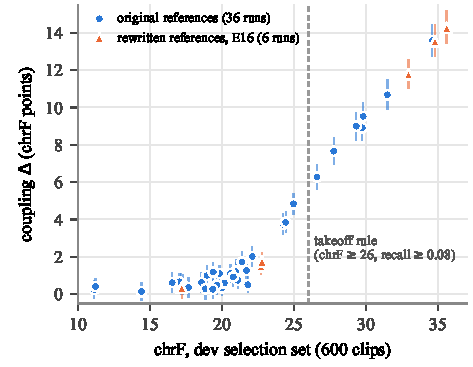
\includegraphics[width=\columnwidth]{fig_runs.pdf}
\caption{All 42 from-scratch runs at epoch 10 on the dev selection set. Error bars are 95\% bootstrap intervals over clips. Runs fall into two groups with nothing between chrF 25 and 26.5. Coupling rises with chrF ($r=0.93$) but separates runs the binary rule cannot, for example partial runs at $\cpl$ 3.7--4.8. The triangles are E16, trained on rewritten references (\S\ref{sec:refs}).}
\label{fig:runs}
\end{figure}

\paragraph{One configuration, three outcomes.}
Our first experiment (E3) compared five input pipelines, one seed each. Upstream Uni-Sign preprocessing led at 29.8 chrF against 18.3--22.9 for the others, and the obvious reading was that compatibility with the pretrained weights matters. Three seeds of the winning configuration then scored 29.8, 21.0 and 19.8. Every other arm fell inside that spread, so we withdrew all five comparisons. The training curves show why. All runs follow one path through epoch 4; the run that succeeds leaves it at epoch 5 and ends at a dev cross-entropy of 2.29, while the others flatten at 2.69--2.75 and cycle through a few stock broadcast phrases. In the worst case, one sentence (``now let us turn to the main news that shook the world'') is emitted for 140 of 600 clips; it is the most repeated reference in the training set. ``Seed'' here labels a run rather than reproducing it: under the default non-deterministic kernels, two runs with seed 0 reached losses of 18.34 and 17.26 by batch 400.

\paragraph{What we varied.}
Table~\ref{tab:arms} lists every from-scratch arm, each judged against the three baseline seeds (B). The arms covered each place a lever could plausibly sit:
\begin{itemize}[leftmargin=*,itemsep=1pt,topsep=2pt]
\item \emph{encoder objective}: InfoNCE \citep{oord2018cpc} between pooled pose embeddings and a frozen mT5 text embedding (E5), and a token-level version (E6);
\item \emph{optimisation}: mT5 slower than the encoder (E4), and the encoder twice as fast (E4b);
\item \emph{decoder initialisation}: mT5 domain-adapted by span corruption \citep{raffel2020t5} on our training transcripts, cutting held-out perplexity from 15.5 to 4.6 (E7);
\item \emph{temporal input}: all sources resampled to a common 12.5 or 15 fps (E9, E9b), native frame rate (E10), and native rate capped Uni-Sign-style at 256 randomly sampled frames (E11);
\item \emph{data}: the 4{,}200 audit-flagged \qz{} references removed (E13; \S\ref{sec:refs}).
\end{itemize}

\begin{table}[t]
\centering\small
\setlength{\tabcolsep}{3pt}
\resizebox{\columnwidth}{!}{%
\begin{tabular}{llcll}
\toprule
Arm & Change & Takeoff & Takeoff chrF & $\cpl$ fail \\
\midrule
B & baseline & 1/3 & 29.8 & 1.19 \\
E4 & mT5 LR $\div10$ & 0/3$^\dagger$ & -- & 0.52 \\
E4b & encoder LR $\times2$ & 2/6 & 29.7, 31.5 & 1.29 \\
E5 & seq.\ alignment & 0/3 & -- & 1.49 \\
E6 & token alignment & 1/3 & 29.3 & 1.41 \\
E7 & adapted mT5 & 0/1 & -- & 0.28 \\
E9 & 12.5 fps & 0/2 & -- & 0.55 \\
E9b & 15 fps & 2/6 & 34.6, 27.7 & 0.90 \\
E10 & native fps & 0/3 & -- & 0.30 \\
E11 & native, cap 256 & 1/3 & 26.6 & 0.63 \\
E13 & drop flagged refs & 0/3 & -- & 2.98 \\
\midrule
\multicolumn{2}{l}{all, original refs} & 7/36 & 26.6--34.6 & \\
E16 & rewritten refs & 3/6 & 35.6/34.8/32.9 & 1.20 \\
\bottomrule
\end{tabular}}
\caption{From-scratch arms (dev selection set, epoch 10). $\cpl$ fail is the mean coupling of runs that did not take off. $^\dagger$E4 is undertrained (train CE 3.33--3.36 against the baseline's 2.12--2.50) and cannot be classified. Per-run numbers are in Appendix~\ref{app:runs}.}
\label{tab:arms}
\end{table}

\paragraph{None of them moved the rate.}
Across the 36 runs on the original references, 7 took off (19\%). No arm differs from baseline in takeoff rate, and at these sample sizes none could have shown a moderate change. More useful is what each arm did to the quantity it was meant to change. Both alignment arms drove their contrastive loss from chance (5.58) to 1.2--2.0: the encoder learned to identify its own transcript, and the decoder still did not use it. The adapted decoder fitted the text faster (train CE 4.1 against 5.0 after one epoch) and then collapsed onto the same stock phrase as the failed baselines. Twice we reported a ceiling or a rate change from a small sample, and twice more seeds removed it. E4b's 2/3 became 2/6. E9b's first takeoff reached 34.6 chrF and coupling 13.6, outside every earlier run, but its next takeoff landed at 27.7 and 7.7, below every earlier run. We keep both corrections in the record because they are the reason the protocol above exists.

\paragraph{The frame-rate series.}
Clips were taken at every second frame on the assumption that all videos were 50 fps; only \ib{} is. Correcting this made results worse. At native rate (E10) every coupling interval includes zero and one seed emits one sentence for 60\% of clips. Uni-Sign never fed its encoder more than 256 frames, and capping native-rate clips at 256 random frames (E11) recovers about half the loss. Lowering the rate everywhere (E9) also hurt. Stride 2, which keeps clips at 220--390 frames, remains the best setting we have tested. The likeliest reading is that the pretrained encoder works best near the sequence statistics it was trained on. That reading was formed after the fact and is untested.

\subsection{Coupling is graded below the threshold}
\label{sec:coupling}

Takeoff is a binary outcome with a base rate near 20\%, so detecting a change from one third to two thirds would take more seeds than we could afford. The coupling measure gives each run a value with its own interval. At the corpus level it adds little: over non-degenerate runs the shuffled score is nearly constant (18.5--21.1 chrF), so corpus $\cpl$ is almost clean chrF minus a constant. That constant is informative in itself. It is the chrF of the text prior, and every run that did not take off scores at or just above what a good run scores with its encoder switched off.

Paired per clip, the measure has resolution the binary rule lacks. Eleven of the first fifteen non-takeoff runs have intervals that exclude zero, so they read their encoder a little. Alignment raised coupling in the failed runs (1.41--1.49 against 1.19), as intended, but never enough to cross the threshold. Slowing the decoder (E4) lowered it to 0.52. Partial runs sit between the groups (E4b\_s5: chrF 24.2, $\cpl$ 3.74). The measure also ranks runs the rule treats as equal: two takeoffs of the same arm, E9b, have non-overlapping intervals (13.6 vs 7.7).

\subsection{Retrieval works where generation does not}
\label{sec:retrieval}

\begin{table}[t]
\centering\small
\setlength{\tabcolsep}{2.5pt}
\begin{tabular}{llrrrr}
\toprule
Task & Source & top-1 & top-5 & MRR & chance \\
\midrule
T1 & Inf. & 0.835 & 0.930 & 0.882 & 0.005 \\
(200-way) & Kha. & 0.885 & 0.945 & 0.910 & 0.005 \\
 & Qaz. & 0.700 & 0.780 & 0.745 & 0.005 \\
 & all & \textbf{0.807} & 0.885 & 0.845 & 0.005 \\
\midrule
T2 & Inf. & 0.900 & -- & 0.939 & 0.162 \\
(own & Kha. & 0.965 & -- & 0.979 & 0.175 \\
broadcast) & Qaz. & 0.639 & -- & 0.749 & 0.147 \\
 & all & \textbf{0.825} & -- & 0.882 & 0.161 \\
\bottomrule
\end{tabular}
\caption{Retrieval on the test split with B\_s0 (original references), opened once. The checkpoint was chosen on dev by T2 MRR under a fixed rule: three takeoff checkpoints were within 0.008, inside a pre-set tie band, so the tie went to the default pipeline. Raw likelihood without the prior correction gives T1 top-1 0.005--0.015.}
\label{tab:retrieval}
\end{table}

Generation asks the model to get every word right from weak, partial evidence, and it loses that contest to the text prior. Retrieval only asks it to rank, and a few correctly read signs (a name, a number, a place) can single out one sentence. Scored as retrieval, the baseline takeoff checkpoint B\_s0, whose generated output has WER 0.96, ranks the right sentence first among 200 for 81\% of test clips, with median rank 1 (Table~\ref{tab:retrieval}). The signal appears only after correcting for the text prior: raw likelihood is at chance. Three controls on dev rule out shortcuts.
(i) \emph{Duration.} Ranking by length match, with a length model fitted on the evaluation clips themselves, gives top-1 0.010.
(ii) \emph{Memorisation.} The nearest training sentence shares a median 9--12\% of content words with a dev reference, and 1 of 400 queries reaches 50\%.
(iii) \emph{Coupling.} The non-takeoff seed B\_s1 ($\cpl=1.27$) reaches 0.015 top-1 where B\_s0 ($\cpl=9.52$) reaches 0.855, so retrieval requires a model that reads its input.
A second takeoff checkpoint from another arm (E4b\_s1) replicates the result at 0.850. \qz{} is the weak source in both tasks, by 0.2--0.3. The next section shows why.

\subsection{The references were the bottleneck}
\label{sec:refs}

\paragraph{Retrieval as an auditor.}
We score every clip in a broadcast against every sentence of that broadcast and flag a \emph{mutual mismatch} when another sentence fits the clip better and the clip's own sentence fits another clip better. This is stricter than a single ranking error, which is often ordinary model error. Over 16{,}174 dev and test clips, 0.4\% of \kh{} and 1.5\% of \ib{} clips are flagged, against 11.5\% of \qz{}. On the 58{,}437 training clips the figures are 0.4\%, 1.0\% and 13.1\% (4{,}200 clips). B\_s0 retrieves its own training clips no better than unseen dev clips (\qz{} 0.689 vs 0.670), so it has not memorised its training pairs and can audit them directly. The flags were checked against a signal the model never sees, implied speech rate. Clips whose transcript implies fewer than 1 or more than 4 words per second are flagged 9.8 times as often on train and 12.5 times on dev. The source of the problem is the article matching: within \qz, clips with \texttt{text\_human} references are flagged 2.8 times as often as clips with \texttt{text\_asr}, and 3.9 times in long broadcasts. This holds even though the ASR clips come from larger broadcasts, which makes retrieval harder for them.

\paragraph{Removing the flagged references does nothing.}
Training from scratch without the 4{,}200 flagged clips (E13) gave no takeoff in three seeds and no \qz-specific change in partial runs. To remove the takeoff lottery, E14 fine-tuned B\_s0 for three epochs on four datasets: cleaned, minus 4{,}200 \emph{random} \qz{} clips, and two identical full copies, which give the noise floor. Removing the flagged clips and removing random ones differ by $-0.003$ on \qz{} T2 top-1, against a measured threshold of 0.044, and neither differs from full data. Dropping a misaligned reference also drops its clip, and the remaining references are loose in a way the conservative flag does not catch.

\paragraph{Rewriting them.}
The two \qz{} transcripts fail in opposite ways: the ASR has the right boundaries and noisy words, and the article has the right words and the wrong boundaries. We give Qwen3.6-27B \citep{qwen36}, served with vLLM \citep{kwon2023vllm} using greedy decoding and thinking off, the clip's ASR and the article text of the clip and its two neighbours on each side. We ask it to write exactly the ASR's span in the article's wording (prompt in Appendix~\ref{app:prompt}). It never sees the current reference. A guard, fixed on a 600-clip dev pilot before the full run, accepts a rewrite only if its length is within $[0.67, 1.5]\times$ that of the ASR, with Whisper's duplicated passages collapsed, and its chrF against the ASR is at least 45. Rejected clips keep their reference. On 34{,}768 clips, which took 72 minutes on two GPUs, 96.5\% of train and 97.0\% of dev rewrites were accepted. Median chrF between rewrite and original is 93, and 7.9\% fall below 30, which means nearly replaced.

\paragraph{Most of the \qz{} deficit was evaluation error.}
B\_s0 never saw dev, so it can judge which version of a dev reference fits the signing (Table~\ref{tab:precheck}). Rewriting only \qz's dev references, with the model unchanged, raises its T2 top-1 from 0.670 to 0.869 and lowers its mutual-mismatch rate from 20.4\% to 6.2\%. Of the 0.30 gap to \kh, 0.20 was in the references. This is not a length effect: rewritten references are longer on average, but the gain is also large where the rewrite is shorter (0.705 to 0.803), and it grows with how much the text changed. The 39 references that were nearly replaced go from 10\% to 85\% retrievable.

\begin{table}[t]
\centering\small
\setlength{\tabcolsep}{4pt}
\begin{tabular}{lrrrr}
\toprule
Dev refs & Inf. & Kha. & Qaz. & mismatch \\
\midrule
original & 0.925 & 0.967 & 0.670 & 20.4\% \\
LLM-rewritten & 0.925 & 0.967 & \textbf{0.869} & 6.2\% \\
raw ASR & 0.925 & 0.967 & 0.877 & 6.2\% \\
\bottomrule
\end{tabular}
\caption{T2 dev top-1 of a fixed model (B\_s0) under three versions of the \qz{} dev references (Inf./Kha./Qaz.\ = \ib/\kh/\qz; mismatch is the \qz{} mutual-mismatch rate). The other sources are untouched, and their scores do not move.}
\label{tab:precheck}
\end{table}

\paragraph{Training on rewritten references.}
Fine-tuning B\_s0 on rewritten training references (E15, two seeds) raised \qz{} chrF by 3.2 against the two identical full-data arms, which differ from each other by 0.28. \ib{} and \kh{} stayed within their spread, and the \qz{} output/reference length ratio rose from 0.84 to 0.97: trained on fragments, the model had learned to stop early. The pre-registered retrieval measure moved by $+0.011$, under its bar of 0.044, because a coupled model is already near its retrieval ceiling. Training from scratch on the rewritten references (E16, six seeds; dev and test references left original) is the only from-scratch arm that changed the level of the good mode. Its three takeoffs reach 35.6, 34.8 and 32.9 chrF, against 26.6--34.6 for every takeoff on the original data (mean 29.9), and coupling 11.8--14.3 against 6.3--13.6. Gains appear in every source, not only the cleaned one, and \qz{} now scores above \ib. The takeoff rate, 3/6 against 7/36, is not significantly different ($p=0.13$).

\begin{table*}[t]
\centering\small
\setlength{\tabcolsep}{3.6pt}
\begin{tabular}{lrrrrrrrrcc}
\toprule
& \multicolumn{6}{c}{Generation (600-clip test selection set)} & \multicolumn{4}{c}{Retrieval top-1} \\
\cmidrule(lr){2-7}\cmidrule(lr){8-11}
Model & chrF & recall & Inf. & Kha. & Qaz. & $\cpl$ [95\% CI] & T1 & T2 & T1 Qaz. & T2 Qaz. \\
\midrule
B\_s0 & 30.27 & 0.135 & 27.3 & 34.3 & 28.7 & 9.39 [8.62, 10.17] & 0.807 & 0.835 & 0.700 / 0.785 & 0.651 / 0.784 \\
E16\_s0 & \textbf{35.76} & \textbf{0.195} & 31.8 & 39.2 & 36.2 & 13.95 [13.10, 14.80] & \textbf{0.853} & \textbf{0.863} & 0.745 / 0.885 & 0.688 / 0.826 \\
\bottomrule
\end{tabular}
\caption{Test split, original references unless marked. Both checkpoints were fixed on dev before test was opened. Paired bootstrap chrF difference: $+5.49$ [4.90, 6.08]. For the two \qz{} retrieval columns, the values are original / rewritten test references. On rewritten references E16\_s0 reaches chrF 36.18, T1 0.900 and T2 0.912.}
\label{tab:test}
\end{table*}

\paragraph{The result holds on test.}
E16\_s0, the best dev run, was compared on test with the baseline B\_s0 (Table~\ref{tab:test}). The test references were rewritten with the frozen prompt and guard (97.3\% accepted), and both versions are reported. chrF rises by 5.5 [4.9, 6.1], coupling by 4.6, and retrieval in both tasks. The test set has the same reference problem as dev: B\_s0's \qz{} T2 rises from 0.651 to 0.784 when only the references change. Every \qz{} number scored against the original references, including those in this paper's earlier sections, understates the model.

\subsection{What the best model gets wrong}
\label{sec:errors}

\begin{table}[t]
\centering\small
\setlength{\tabcolsep}{5pt}
\begin{tabular}{lrrr}
\toprule
Reference word band & $n$ & B\_s0 & E16\_s0 \\
\midrule
common ($\geq$500 in train) & 4{,}603 & 0.237 & 0.323 \\
mid (20--500) & 7{,}186 & 0.094 & 0.159 \\
rare ($<$20) & 2{,}325 & 0.006 & \textbf{0.026} \\
unseen in train & 530 & 0.000 & 0.000 \\
numbers & 477 & 0.382 & 0.532 \\
\midrule
content-word precision & & 0.148 & 0.201 \\
\bottomrule
\end{tabular}
\caption{Recall of reference words by training frequency, dev selection set. Precision is the share of the hypothesis's content words that appear in the reference.}
\label{tab:bands}
\end{table}

At the median clip the model names the right topic, place or figure in fluent Kazakh and fills the rest with plausible, wrong detail. Table~\ref{tab:bands} makes this concrete. Common words are recovered about a third of the time and numbers about half the time, but rare words only 2.6\% of the time, and 80\% of the model's content words are not in the reference. Most rare words are names and places, which interpreters fingerspell or render with name signs. Here a hand spans 31--51 pixels and adjacent finger joints are 2--3 pixels apart (Table~\ref{tab:data}), so handshape is at the edge of what any keypoint detector can resolve, and better re-detection is impossible because no larger originals exist. The best source on every measure, \kh, is the one with the largest hands. With three sources, that is a hypothesis.

Recall also falls along the sentence. Pose-attributable recall (clean minus shuffled) drops from 0.173 in the first fifth of the reference to 0.080 in the last, a factor of 2.16. The drop is the same in every takeoff run and survives restricting to hypotheses at least as long as their reference. The missing end-of-sentence content does not reappear in the next clip, as interpreter lag would predict (the end-minus-start difference in the adjacent clip is $-0.002$ to $+0.001$, SE $\approx 0.004$). The likeliest explanation is that it was never signed: simultaneous interpreters compress fast news speech. If so, a speech transcript is a ceiling no signing-based model can reach, and part of what looks like model error is reference content with no counterpart in the input. Testing this needs sign-faithful annotation. We have built the annotation tool and a 100-clip package without audio, but no interpreter has worked through it yet.

\section{Conclusion}

We set out to find the best model for translating Kazakh Sign Language news from pose, and most of what we learned is about measurement. Training is a lottery between reading the pose and reciting the prior, and no change we made to the encoder, the optimiser, the decoder's initialisation or the temporal input changed the odds. A paired pose-shuffle measure shows the lottery is not all-or-nothing and gives each run an interval that a takeoff count cannot. The same checkpoints that write poor sentences retrieve the right one 81--86\% of the time, which makes retrieval both a usable task today and a tool for auditing the corpus. The audit found that one source's references often describe the wrong part of the broadcast. Rewriting them with an LLM showed that most of that source's deficit was in the evaluation set, and training on the rewrites gave the study's only large gain, +5.5 test chrF across all sources. The model now gets the story and misses the specifics. With hands 31--51 pixels wide and interpreters who compress what they hear, the remaining gap may lie in the input and the references as much as in the model.

For similar projects we recommend: run at least three seeds before comparing arms, and report coupling with intervals alongside any takeoff count; check every reference set with the model before trusting per-source numbers; prefer rewriting noisy references to dropping them; and treat retrieval as a deliverable whenever candidate text exists, such as the day's articles.

\section*{Limitations}

\textbf{One encoder, one decoder.} All runs use Uni-Sign's pose encoder with mT5-base, and other architectures, larger decoders or RGB input may behave differently. RGB was outside the project's scope. \textbf{Seeds.} Most arms have three seeds, and E7 has one. Takeoff rates near 20\% cannot be compared reliably at that size, so no arm is shown to leave the rate unchanged; we show only that none changed it detectably. \textbf{The rewrite.} The LLM can introduce errors, and the guard checks only length and overlap against the ASR, not meaning. The rewrites have not been checked by a native speaker against the signing. Retrieval on rewritten references improves with how much the text changed, which supports the rewrite but is also measured by a model trained on the old references. \textbf{References are speech, not signing.} Every reference transcribes what the anchor said, and \S\ref{sec:errors} suggests interpreters omit part of it, so all absolute scores mix model error with untranslatable reference content. \textbf{One test set, opened twice.} Each opening used one checkpoint fixed on dev, but the same test clips served both. \textbf{Comparability.} chrF is sacreBLEU's default chrF2 on raw text, so it is case- and punctuation-sensitive, which affects \qz{} (cased and punctuated) more than the other sources. No prior continuous KSL translation result exists to compare against. \textbf{Data access.} The data are broadcast interpretation held under a restricted-access agreement and are not redistributed; interpreters appear in the source videos, and only keypoints were used for training. \textbf{Use of the output.} Output of the quality reported here should not be shown to Deaf viewers as a translation: it invents specific names and places 80\% of the time. Retrieval against known text is the safer use.

\bibliographystyle{plainnat}
\bibliography{refs}

\appendix
\onecolumn

\section{Pipeline faults that would have changed a conclusion}
\label{app:faults}

Each of these ran without an error, and each would have produced a plausible but wrong result. They are listed in the order we found them.

\begin{enumerate}[leftmargin=*,itemsep=2pt]
\item \textbf{Validation never saw two sources.} Generation-based model selection used the first 25 unshuffled batches, and because sources were concatenated in order, all 200 clips came from \ib. \qz{}, 48.6\% of dev, was never generated on. Replaced by the stratified selection set.
\item \textbf{Splits leaked across dataset versions.} Each manifest was internally disjoint, but the archived \qz{} train shared 563 videos with the recollected dev (64\% of dev clips). This invalidated an earlier clean-versus-noisy data experiment.
\item \textbf{Two BLEUs.} The trainer reported normalised BLEU and the evaluator raw BLEU. On identical predictions they gave 63.4 and 30.3, so every BLEU quoted before the fix was normalised and not comparable to published numbers.
\item \textbf{Padding leaked into real frames.} Masking only around the temporal ST-GCN stack let convolution bias and BatchNorm shift reach the last real frames (maximum difference 0.65). Fixed by re-zeroing after each block.
\item \textbf{Wrists were elbows.} The body mapping copied elbow values into the wrist slots.
\item \textbf{The confidence channel was constant.} RTMW scores are $\geq 1$ for 99.6--100\% of joints, so clipping to $[0, 1]$ produced a channel with standard deviation 0. Upstream Uni-Sign clips the same way.
\item \textbf{New heads in no optimiser group.} The alignment heads never trained, and the loss sat at chance.
\item \textbf{A guard that consumed its input.} A check that every parameter had an optimiser group iterated over generator-valued groups and emptied them, so mT5 stopped training. Caught by comparing the loss curve with the baseline's.
\item \textbf{Wrong sentinel IDs.} On our tokenizer version, \texttt{convert\_tokens\_to\_ids('<extra\_id\_0>')} returns \texttt{<unk>}, which would have broken span corruption silently.
\item \textbf{A mislabelled frame rate.} ``Every second frame of a 50 fps video'' was true for only one source (Table~\ref{tab:data}). The E9 smoke test missed this because it built the dataset directly instead of through the trainer's config path.
\item \textbf{A one-sample noise floor.} A first parity test of a rewritten trainer declared a bug at 0.79 loss difference against an old-versus-old gap of 0.13. A second run landed 0.30 on the other side. Deterministic mode then gave exact parity over 400 batches.
\end{enumerate}

\section{LLM rewrite prompt and guard}
\label{app:prompt}

The prompt is given verbatim (version 2, frozen after the dev pilot). \texttt{\{article\}} is the \texttt{text\_human} of the clip and its two neighbours on each side, in time order, with consecutive duplicates removed. \texttt{\{speech\}} is the clip's \texttt{text\_asr}.

{\small
\begin{verbatim}
You are cleaning the reference transcripts of a Kazakh sign-language news corpus.

SPEECH is an automatic speech recognition of exactly what the news anchor said during one
short video clip. Its first and last words are the true boundaries of the clip, but words
can be misrecognised, and it has no capital letters or punctuation.

ARTICLE is the human-written news text for this broadcast, around the clip. Its wording,
spelling, names and numbers are correct, but it is NOT aligned to the clip: it contains
sentences said before and after the clip, and it may lack some things that were said.

Write the transcript of exactly what was said in this clip, in clean written Kazakh:
- Cover the same content as SPEECH, from its first word to its last. Do not add anything
  SPEECH does not contain, and do not drop anything it does.
- Where SPEECH matches the ARTICLE, use the ARTICLE's wording, spelling, capitalisation,
  numbers and punctuation.
- Where SPEECH has no counterpart in the ARTICLE, keep it, fixing only obvious recognition
  errors.
- If SPEECH starts or ends in the middle of a sentence, start or end at the same point.
- Speech recognition sometimes repeats a passage by mistake. If SPEECH contains the same
  passage twice in a row and the ARTICLE has it once, write it once.
- Do not add ellipses or any marks that are not part of the text.

Output only the transcript, nothing else.

ARTICLE:
{article}

SPEECH:
{speech}
\end{verbatim}
}

\noindent\textbf{Guard.} Let $a$ be the ASR with any repeated passage of at least 5 words collapsed, and $r$ the rewrite with ellipses removed. Accept if $0.67 \le |r|/|a| \le 1.5$ in words and $\mathrm{chrF}(r, a) \ge 45$, both computed on lower-cased text with punctuation stripped. On the 600-clip pilot, rejections were 1.8\% for length, 0.5\% for overlap and 0.8\% for a missing ASR or article. Accepted rewrites score chrF 91.8 against the ASR, compared with 72.7 for the original references.

\section{All from-scratch runs}
\label{app:runs}

\begin{table}[H]
\centering\footnotesize
\begin{tabular}{lrrrrrrll}
\toprule
Run & chrF & recall & \ib & \kh & \qz & distinct & $\cpl$ [95\% CI] & takeoff \\
\midrule
B\_s0 & 29.79 & 0.128 & 27.0 & 33.8 & 28.2 & 598 & 9.52 [8.77, 10.29] & yes \\
B\_s1 & 21.02 & 0.031 & 18.5 & 24.2 & 20.0 & 503 & 1.27 [0.66, 1.86] & no \\
B\_s2 & 19.83 & 0.025 & 18.6 & 21.5 & 19.3 & 523 & 1.11 [0.68, 1.56] & no \\
E4\_s0 & 21.10 & 0.023 & 21.2 & 22.9 & 18.8 & 525 & 0.74 [0.32, 1.17] & no \\
E4\_s1 & 21.79 & 0.023 & 22.6 & 22.7 & 19.7 & 558 & 0.50 [0.10, 0.94] & no \\
E4\_s2 & 20.02 & 0.019 & 21.1 & 21.0 & 17.6 & 505 & 0.33 [-0.08, 0.77] & no \\
E4b\_s0 & 29.73 & 0.125 & 27.4 & 33.2 & 28.3 & 600 & 8.91 [8.22, 9.60] & yes \\
E4b\_s1 & 31.47 & 0.145 & 29.2 & 35.2 & 29.6 & 599 & 10.68 [9.90, 11.50] & yes \\
E4b\_s2 & 11.14 & 0.010 & 8.1 & 11.2 & 14.4 & 128 & 0.24 [-0.23, 0.73] & no \\
E4b\_s3 & 17.17 & 0.021 & 14.0 & 20.1 & 17.2 & 300 & 0.54 [-0.02, 1.09] & no \\
E4b\_s4 & 18.56 & 0.019 & 15.6 & 20.7 & 19.3 & 402 & 0.63 [0.08, 1.17] & no \\
E4b\_s5 & 24.24 & 0.059 & 22.3 & 26.8 & 23.4 & 597 & 3.74 [3.19, 4.32] & no \\
E5\_s0 & 21.70 & 0.029 & 20.3 & 23.9 & 20.7 & 566 & 1.26 [0.76, 1.79] & no \\
E5\_s1 & 22.10 & 0.037 & 20.2 & 24.7 & 21.1 & 586 & 2.01 [1.50, 2.56] & no \\
E5\_s2 & 20.95 & 0.025 & 18.3 & 23.7 & 20.6 & 521 & 1.20 [0.69, 1.72] & no \\
E6\_s0 & 21.39 & 0.034 & 19.0 & 24.3 & 20.6 & 567 & 1.72 [1.20, 2.28] & no \\
E6\_s1 & 29.31 & 0.123 & 25.6 & 33.5 & 28.7 & 598 & 9.00 [8.24, 9.72] & yes \\
E6\_s2 & 20.59 & 0.027 & 18.6 & 23.2 & 19.7 & 522 & 1.10 [0.62, 1.57] & no \\
E7\_s0 & 18.85 & 0.018 & 13.5 & 22.5 & 20.2 & 283 & 0.28 [-0.27, 0.82] & no \\
E9\_s0 & 17.29 & 0.015 & 13.9 & 19.2 & 18.7 & 334 & 0.50 [-0.02, 1.07] & no \\
E9\_s1 & 20.18 & 0.021 & 19.2 & 22.4 & 18.6 & 437 & 0.60 [0.14, 1.04] & no \\
E9b\_s0 & 18.96 & 0.025 & 17.4 & 20.5 & 18.9 & 427 & 1.00 [0.42, 1.55] & no \\
E9b\_s1 & 19.39 & 0.025 & 16.9 & 21.9 & 19.2 & 490 & 1.18 [0.65, 1.70] & no \\
E9b\_s2 & 34.57 & 0.181 & 31.8 & 37.8 & 34.0 & 599 & 13.59 [12.75, 14.46] & yes \\
E9b\_s3 & 27.74 & 0.106 & 25.4 & 31.2 & 26.3 & 599 & 7.66 [6.95, 8.40] & yes \\
E9b\_s4 & 20.78 & 0.025 & 19.9 & 22.5 & 19.7 & 528 & 0.92 [0.41, 1.42] & no \\
E9b\_s5 & 19.65 & 0.018 & 18.2 & 22.2 & 18.2 & 394 & 0.49 [-0.02, 1.03] & no \\
E10\_s0 & 14.42 & 0.012 & 16.2 & 11.9 & 15.1 & 133 & 0.13 [-0.34, 0.62] & no \\
E10\_s1 & 11.23 & 0.010 & 8.8 & 11.7 & 13.4 & 107 & 0.40 [-0.04, 0.83] & no \\
E10\_s2 & 17.68 & 0.014 & 13.8 & 19.2 & 20.0 & 231 & 0.35 [-0.20, 0.88] & no \\
E11\_s0 & 17.05 & 0.015 & 9.8 & 21.4 & 19.5 & 250 & 0.65 [0.21, 1.11] & no \\
E11\_s1 & 16.55 & 0.016 & 11.2 & 19.3 & 18.9 & 227 & 0.62 [0.10, 1.14] & no \\
E11\_s2 & 26.59 & 0.091 & 24.9 & 29.5 & 25.1 & 598 & 6.27 [5.62, 6.92] & yes \\
E13\_s0 & 24.96 & 0.068 & 22.5 & 27.8 & 24.4 & 595 & 4.83 [4.25, 5.41] & no \\
E13\_s1 & 24.42 & 0.061 & 22.6 & 26.8 & 23.7 & 588 & 3.85 [3.31, 4.41] & no \\
E13\_s2 & 19.36 & 0.019 & 15.6 & 22.0 & 20.3 & 347 & 0.26 [-0.26, 0.76] & no \\
E16\_s0 & 35.57 & 0.191 & 32.3 & 38.4 & 36.0 & 599 & 14.26 [13.40, 15.17] & yes \\
E16\_s1 & 22.70 & 0.034 & 20.8 & 24.1 & 23.2 & 579 & 1.50 [1.03, 1.98] & no \\
E16\_s2 & 34.76 & 0.183 & 30.8 & 37.6 & 35.9 & 598 & 13.55 [12.71, 14.44] & yes \\
E16\_s3 & 32.92 & 0.160 & 28.7 & 36.1 & 34.0 & 598 & 11.79 [11.03, 12.59] & yes \\
E16\_s4 & 22.77 & 0.036 & 20.6 & 24.6 & 23.0 & 586 & 1.74 [1.26, 2.24] & no \\
E16\_s5 & 17.20 & 0.017 & 12.0 & 20.1 & 19.3 & 320 & 0.34 [-0.26, 0.92] & no \\
\bottomrule
\end{tabular}
\caption{Every from-scratch run at epoch 10 on the dev selection set (600 clips, original references), scored through one metric path. ``Distinct'' is the number of different hypotheses among 600. Contamination (evaluation videos seen in training) is 0 for every run.}
\end{table}

\section{Decoding sweep}
\label{app:decode}

The sweep used a single checkpoint on the dev selection set and crossed beam $\{1, 4\}$, repetition penalty $\{1.0, 1.1, 1.3\}$ and trigram blocking on/off. With beam 1 all six settings scored 34.69--34.96 chrF; with beam 4, 36.00--36.27. Beam 4 is consistently better, and the penalty and blocking settings make no difference. The checkpoint for this sweep came from an initialiser excluded from the paper (Appendix~\ref{app:excluded}), so only the relative differences are used.

\section{Excluded results}
\label{app:excluded}

An mT5 checkpoint fine-tuned by a colleague on an earlier version of this corpus reached 36.25 chrF and 0.207 recall on the clean subset of the selection set. We exclude it because its training history is unrecorded and may overlap our dev and test videos. All results in the paper start from public weights (Uni-Sign CSL stage 1 and \texttt{google/mt5-base}). Earlier prosody and speech-synthesis stages, and an RGB fusion branch, were dropped for scope; their code is in the project history.

\section{Compute}

Each from-scratch run took about 5.7\,h, and a fine-tune about 1.5\,h, on one NVIDIA RTX PRO 6000 (96\,GB). The 42 from-scratch runs account for roughly 240 GPU-hours. Scoring a checkpoint on the selection set takes about 40\,s, plus the same again for the shuffled pass, and the LLM rewrite of 34{,}768 clips took 72 minutes on two GPUs.

\end{document}
